\documentclass[unknownkeysallowed, 10pt, a4 paper, handout]{beamer}

% Custom beamer theme
\usepackage{../style/beamerthemeCustom}
\newcommand{\HRule}{\rule{\linewidth}{0.5mm}}   %FOR TITLEPAGE

\usepackage{changepage}       % adjustwidth

\setlength\parskip{0.3cm}

\definecolor{darkgreen}{RGB}{0,100,0}
\newcommand{\green}[1]{\textbf{\textcolor{darkgreen}{#1}}}
\newcommand{\red}[1]{\textbf{\textcolor{red}{#1}}}

\newcommand{\focus}[1]{\textbf{\textcolor{red}{#1}}}
\newcommand{\ra}{$\longrightarrow$ }
\newcommand{\lra}{$\longleftrightarrow$ }

\newcommand{\code}[1]{\colorbox{black}{\color{green}\texttt{#1}}}

% Command to create two side-by-side minipages
\newcommand{\sidebyside}[5]{
  \begin{minipage}{#1\textwidth}
    #2
  \end{minipage} #3 \begin{minipage}{#4\textwidth}
    #5
  \end{minipage}
}

\begin{document}

\begin{frame}
  \begin{center}

    \definecolor{myblue}{RGB}{51,51,179}
    \setbeamercolor{block body}{use=structure,fg=white,bg=myblue!20!myblue}

    \begin{block}{}
      \Large
      \centering
      Linux Basics IV:\\
      Basic shell scripting
    \end{block}

    \vspace{6mm}
    \large
    \textsc{Adriano Angelone, Graziano Giuliani} \\

  \end{center}
\end{frame}

\begin{frame}[label=outline]{Course Outline}
  \begin{itemize}
    \item UNIX/Linux Basics
    \item Intermediate shell commands
    \item Editing and compiling source code
    \item Text file manipulation
    \item \focus{Basic shell scripting}
  \end{itemize}

  \vspace{6mm}

  \centering
  Download slides and exercise files with the command\\
  \code{git clone https://github.com/AA24KK/LinuxBasics.git}\\
  \vspace{1mm}
  or download a ZIP archive at
  \vspace{1mm}
  \code{https://github.com/AA24KK/LinuxBasics/archive/master.zip}

  \vspace{2mm}

  Adriano: \focus{aangelon@ictp.it}, Room 263, ICTP\\
  Graziano: \focus{ggiulian@ictp.it}

\end{frame}

\begin{frame}
  \begin{center}
    \frametitle{Why shell scripting}

    Reuse multiple times the same command:\\
    \focus{less work, less bugs}

    What are the basics:
    \begin{itemize}
      \item Variables
      \item Conditionals
      \item Loops
      \item Arithmetic operations
    \end{itemize}
  \end{center}
\end{frame}


\begin{frame}
  \begin{center}
    \frametitle{Variables}

    Variables contain data\\
    they have a label (\focus{name}) and a \focus{content}

    \begin{center}
      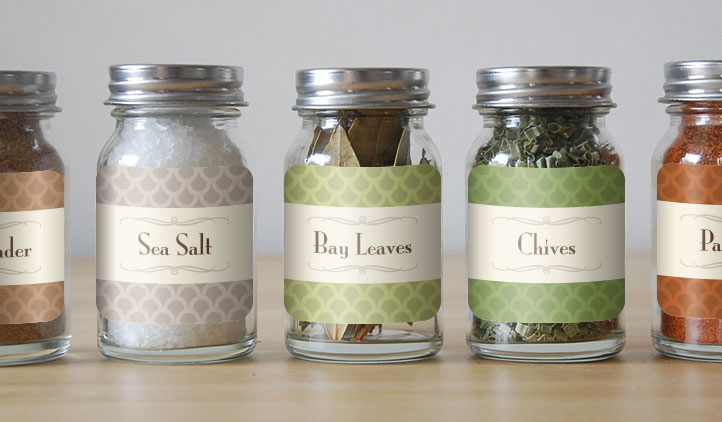
\includegraphics[width=0.72\textwidth]{pics/jars.jpg}
    \end{center}

    In bash, variables \focus{have no type}:\\
    \focus{everything is a string, with arithmetic sometimes possible}
  \end{center}
\end{frame}


\begin{frame}
  \begin{center}
    \frametitle{How to use variables}

    Variables are initialized when you use them the first time:\\
    \focus{you can call non-existing variables}, usually trouble\\
    (unless you put \code{set -u} in your script)

    \sidebyside{0.50}{
      \centering
      \focus{Assignment}: give a variable a value\\
      \code{<variable name>=<value>}

      \vspace{3mm}

      \focus{Expansion}: access the value\\
      \code{\$<variable name>}
    }{\hfill}{0.45}{
      \begin{center}
        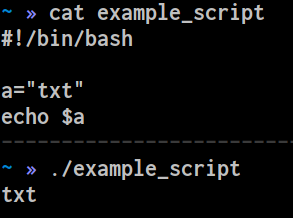
\includegraphics[width=0.70\textwidth]{pics/variables_1.png}
      \end{center}
    }

    Usually it's good to use \code{"\$<variable name>"}\\
    to avoid problems if variable contains spaces

    \sidebyside{0.50}{
      \centering
      Easy to join\\
      variable values and strings

      \vspace{2mm}

      Use \code{\$\{<variable name>\}}\\
      to avoid expanding another variable
    }{\hfill}{0.45}{
      \begin{center}
        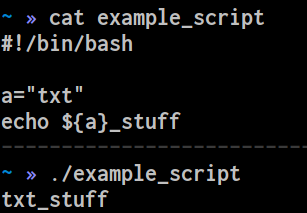
\includegraphics[width=0.70\textwidth]{pics/variables_2.png}
      \end{center}
    }
  \end{center}
\end{frame}

\end{document}
